\section{Introduction}
\begin{frame}{Motivation}%{A Sub-title is optional}
\begin{itemize}
\item Software applications change all the time
\item Deployed systems must be updated with bug fixes, new features
\item Updating typically involves: stop, apply patch, restart
\end{itemize}
\end{frame}

\begin{frame}{}%{A Sub-title is optional}
\begin{textblock*}{0mm}[0,0](5mm,5mm)
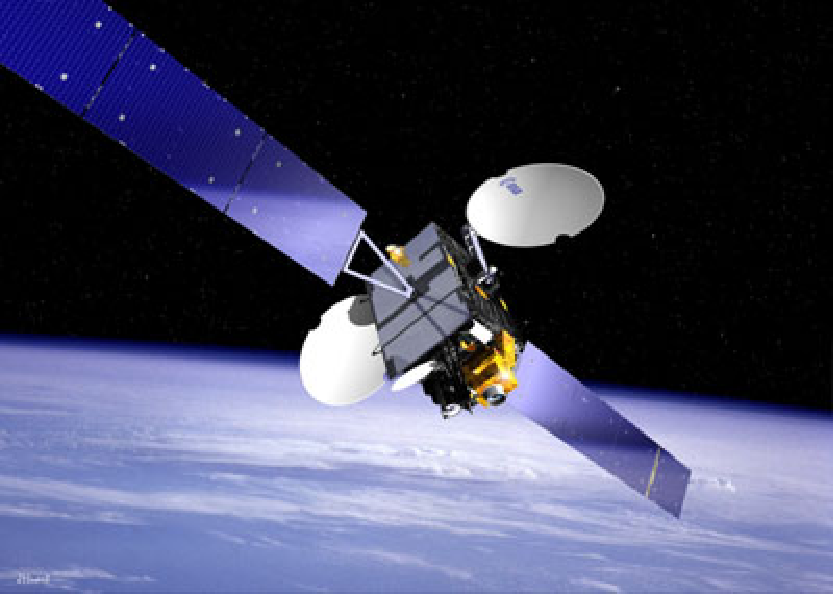
\includegraphics[scale=0.5,clip=true,angle=15,trim=0 30 35 0]{images/3rdparty/esa-satellite}%
\end{textblock*}
\only<2->{\begin{textblock*}{0mm}[0,0](10mm,55mm)
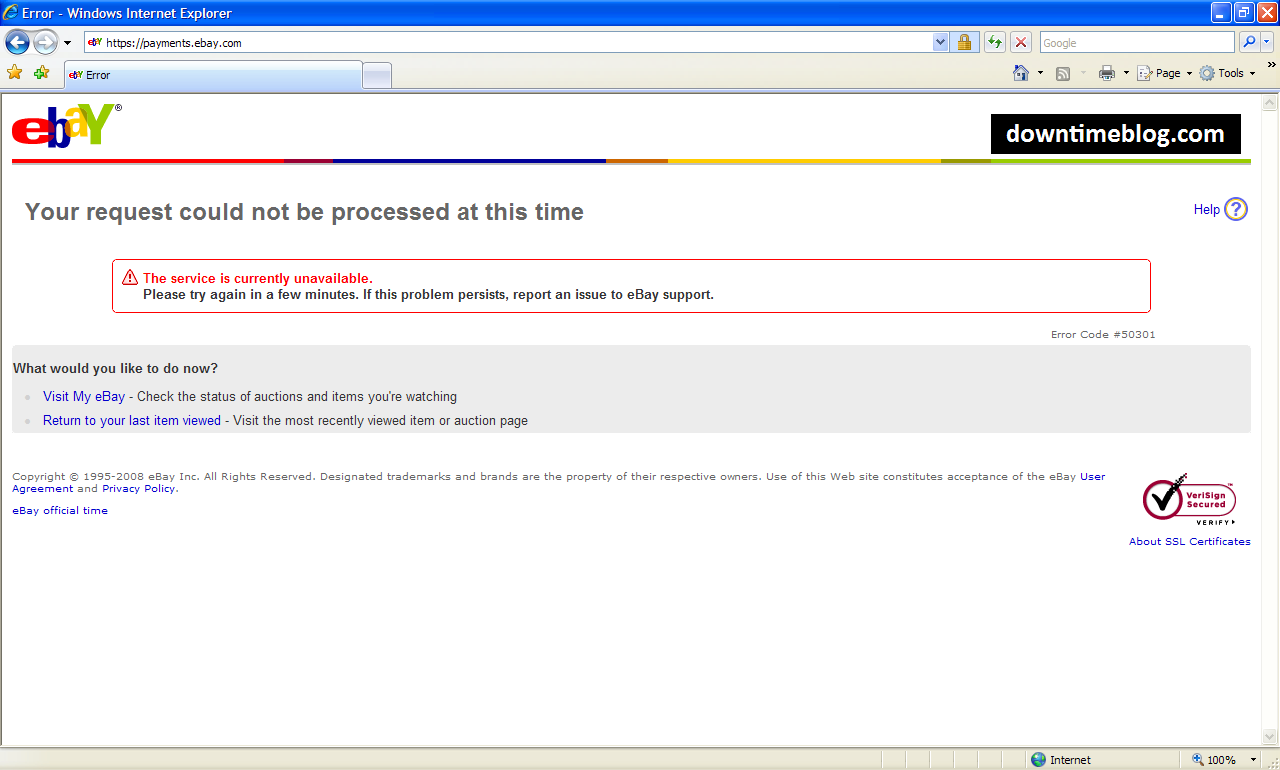
\includegraphics[scale=0.4,clip=true,trim=0 450 525 90]{images/3rdparty/ebay-downtime}%
\end{textblock*}}
\only<3->{\begin{textblock*}{0mm}[0,0](40mm,25mm)
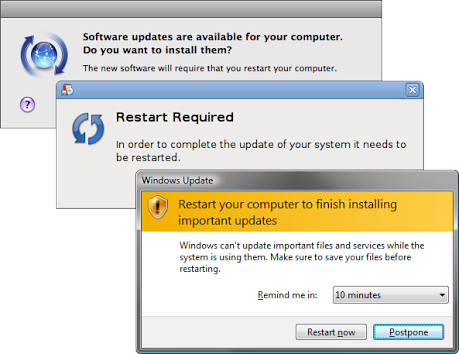
\includegraphics[scale=0.6,clip=true]{images/3rdparty/restart-required}%
\end{textblock*}}
\end{frame}

\begin{frame}{Dynamic Software Updating in the real world}%{A Sub-title is optional}
\only<1>{\begin{textblock*}{0mm}[0,0](24mm,38mm)
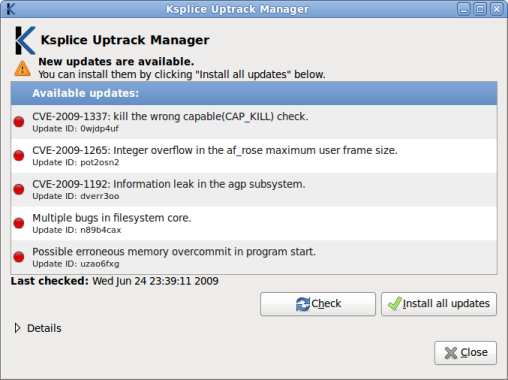
\includegraphics[,clip=true,scale=0.3,angle=345]{images/3rdparty/ksplice}%
\end{textblock*}}
\only<1>{\begin{textblock*}{0mm}[0,0](64mm,6mm)

\includegraphics[,clip=true,scale=1.00,angle=330]{images/3rdparty/erlang}%
\end{textblock*}}
\only<1>{\begin{textblock*}{0mm}[0,0](00mm,00mm)

\includegraphics[,clip=true,scale=0.35,angle=30,trim=0 0 420 0]{images/3rdparty/jetpack}%
\end{textblock*}}
\only<2>{\begin{textblock*}{0mm}[0,0](20mm,30mm)
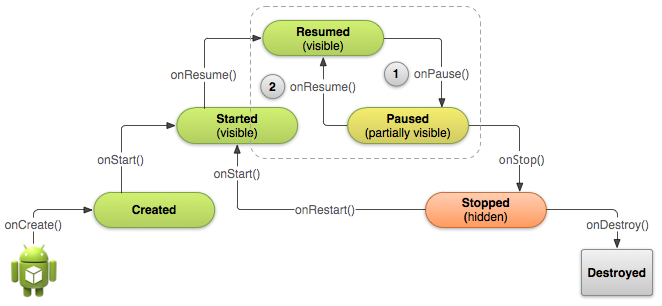
\includegraphics[,clip=true,scale=0.35,angle=0]{images/3rdparty/android-lifecycle}%
\end{textblock*}}
\end{frame}

\begin{frame}{}%{A Sub-title is optional}
\begin{block}{}
\begin{center}
{\LARGE
The fundamental problem is losing state because of downtime.
}
\vspace{0.5ex}
\end{center}
\end{block}
\end{frame}

\begin{frame}{Dynamic software updating}%{A Sub-title is optional}
\vspace*{-3mm}%
\begin{center}%
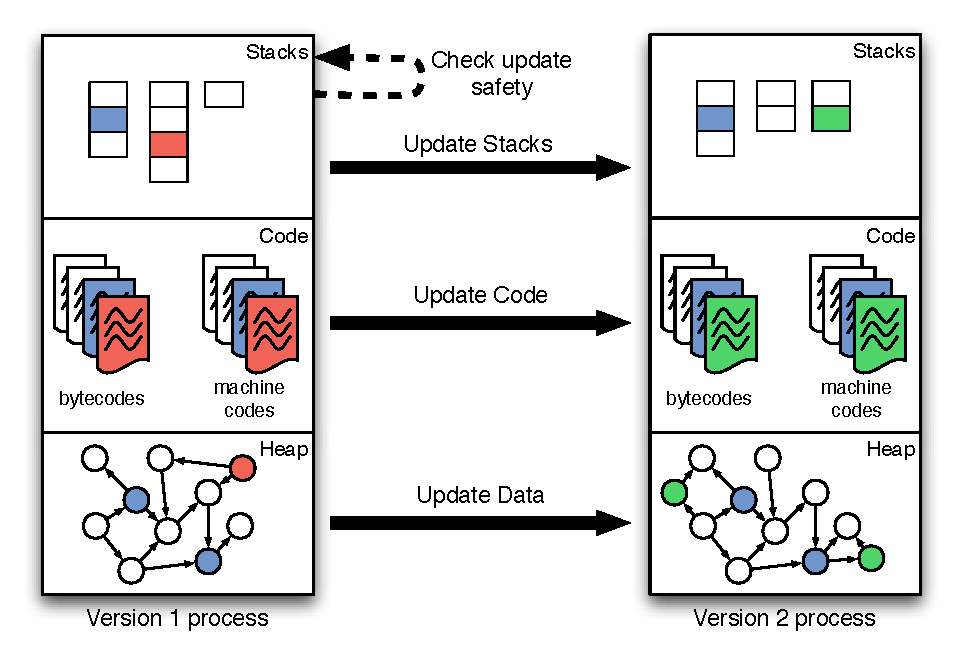
\includegraphics[scale=0.73]{images/process-state/both-process-state}%
\end{center}%
\end{frame}

% \begin{frame}{Dynamic updating systems}%{A Sub-title is optional}
% \begin{itemize}
% \item Special-purpose architectures, application-specific solutions exist
% \item General-purpose solutions gaining strength
%   \begin{itemize}
%   \item K42, Ksplice for OS updates
%   \item Polus, Ginseng for C applications
%   \end{itemize}
% \item Not for managed languages
% \end{itemize}
% \end{frame}

% \begin{frame}{Contribution}%{A Sub-title is optional}
% \begin{itemize}
% \item \DSU{} - A Java Virtual Machine with DSU support
% \item Extend existing VM services
% \item A DSU system that is
%   \begin{description}
%   \item[Safe]
%   \end{description}
% \end{itemize}
% \end{frame}

\begin{frame}{Key contribution}%{A Sub-title is optional}
\DSU{} - a DSU-enabled Java Virtual Machine \\
\begin{description}
\item[Safe] Guarantees type-safe updates\\
              Relies on programmer for semantic-correctness
\item[Flexible] Supports method body and signature changes\\
                   across class hierarchies
\item[Efficient] No overhead during normal execution
\item[Easy to use] The stock application is DSU-ready\\
                   No rewriting/recompilation required
\end{description}
\end{frame}

% \begin{frame}{Our solution}%{A Sub-title is optional}
% \begin{itemize}
% \item \DSU{} - a Java Virtual Machine with DSU support
% % \item Built on top of Jikes RVM, a Java-in-Java VM
% \item Key insight: Extend existing VM services
% %   \begin{itemize}
% %   \item Classloading
% %   \item Bytecode verification%\footnote{Jikes RVM does not have a bytecode verifier}
% %   \item Thread synchronization
% %   \item JIT Compilation
% %   \item On-stack replacement
% %   \item Garbage collection
% %   \end{itemize}
% \item No DSU-related overhead during normal execution
% \item Support updates to real world applications
% \begin{block}{}
% \emph{Dynamic software updating in managed languages can be achieved in a
% {\bf flexible}, {\bf safe}, and {\bf efficient} manner by extending
% existing VM services.}
% \end{block}
% 
% \begin{block}{}
% \emph{DSU support should be a standard feature of future VMs.}
% \end{block}
% \end{itemize}
% \end{frame}
